\documentclass
[answers]
{exam}

\linespread{1.1}

\usepackage{amsmath, amssymb, amsthm}  %% 數學符號用txfonts
\usepackage{mathrsfs} 
%\usepackage{pstricks,pstricks-add} % 引入 pstricks 和 pstricks-add 套件 (繪圖套件) 
%插入GGB圖片===================================
\usepackage{pgf,tikz}
\usepackage{mathrsfs}
\usetikzlibrary{arrows}
%=============================================
\usepackage{graphicx}   %% 插入圖片用
\usepackage{float}  %%強制插入圖片位置
\usepackage{caption}
\usepackage{subfigure}
\usepackage{color}
%\usepackage{minitoc}   %chapter下的小目錄
\usepackage{colortbl}
\usepackage{nopageno}
\usepackage{cases}
\usepackage{textcomp}             % for \textcelsius
\renewcommand{\arraystretch}{1.2} % 將表格行間距加大為原來的 1.2 倍
\arrayrulewidth=1pt               % 調整線條粗細為 1pt
\tabcolsep=15pt                   % 調整欄間距為 24pt


%\begin{figure}[h]
%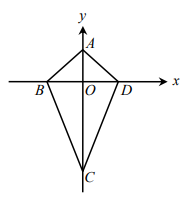
\includegraphics[scale=1.2]{./figure/2.png}
%\end{figure}

\usepackage{wrapfig}  %%圖文並排

%\begin{wrapfigure}{r}{6cm}  r:圖片靠右  6cm:離右邊6cm
%	\centering  圖片在右邊區塊的中間
%	\includegraphics[scale=0.6]{./figure/19.png}
%\end{wrapfigure}

\usepackage{tcolorbox}  %% 顏色方框
\usepackage{tikz}  %%繪製流程圖、腦圖...
\usepackage{array}  %%陣列
\usepackage{booktabs} %調整表格線與上下內容的間隔
\usepackage{multirow}
\usepackage{enumitem}
%可改enumerate的label
\usepackage{tasks}  %%選擇題
\settasks{label=(\Alph*),
		  label-width=3.5ex,
		  label-offset={0.4em},
		  label-align=left,
		  column-sep={1pt},
		  item-indent={21pt}, %%選項前後
		  before-skip={-0.7em},
		  after-skip={-0.7em}}
%[label=(\Alph*),label-width=4ex]  
%\Alph* 選項ABCD  \alph* 選項abcd  \arabic* 選項1234 \roman*羅馬數字
\usepackage{framed}  %%框框
%出入單行字加框  \framebox[\width]{我是一段话}

%插入圖片 \rightline{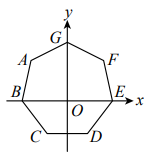
\includegraphics[scale=1.2]{./chapter_1/figure/1.png}}
\usepackage{diagbox}  %%斜線表格頭
\usepackage{ulem}
%\sout{文字} 刪除線		\uwave{文字} 波浪線
%\xout{文字} 斜刪除線		\uuline{文字} 雙下划線
\usepackage[margin=2cm]{geometry} %邊界設定
\usepackage[export]{adjustbox} %插入圖片
\usepackage[colorlinks=true,linkcolor=blue]{hyperref}
%%[是否開啟目錄顏色,目錄顏色設定]{超連結}

%\usepackage{fancyhdr}  %%這兩行是頁首頁尾
%\pagestyle{fancy}  %%頁首頁尾格式
%\fancypagestyle{plain}{}
%\renewcommand{\headrulewidth}{0.4pt}  %%頁首下方直線厚度
%\cfoot{觀念解數學--~\thepage~--態度解人生}
%\fancyhead{} % 清除所有頁首設定
%\fancyhead[RO,LE]{\thechapter}
%\fancyfoot{} % 清除所有頁尾設定
%\fancyfoot[LE,RO]{第~\thepage~頁}      % 頁碼放在偶數頁的左邊及奇數頁的右邊
%\fancyfoot[LO,CE]{奇數頁左及偶數頁中}
%\fancyfoot[CO,RE]{奇數頁中及偶數頁右}
% Texmaker使用者: 上方選擇XeLaTeX後再編譯
\usepackage{xeCJK}   % Chinese input settings
\setCJKmainfont{標楷體} % Windows使用者請使用這行
\setmainfont{Times New Roman}
\defaultCJKfontfeatures{AutoFakeBold=0.5,AutoFakeSlant=0} %以後不用再設定粗斜
\newCJKfontfamily\WC{華康行楷體W5}                       
\XeTeXlinebreaklocale "zh"
\XeTeXlinebreakskip = 0pt plus 1pt
%%上兩行才能讓中文自動換行
\makeatletter
\def\rightharpoonfill@{\arrowfill@\relbar\relbar\rightharpoonup}
\newcommand{\vect}{\mathpalette{\overarrow@\rightharpoonfill@}}
\makeatother
%向量

%\renewcommand{\qedsymbol}{}
\newcommand{\R}{\mathbb{R}} %mathbb 雙行粗體
\newcommand{\Z}{\mathbb{Z}}
\newcommand{\Q}{\mathbb{Q}}
\newcommand{\N}{\mathbb{N}}
\renewcommand{\S}{\mathbb{S}}
\newcommand{\f}{\ensuremath{\mathcal{F}}} 
%%\ensuremath  非數學模式自動加上$符號
\newcommand\norm[1]{\left\lVert#1\right\rVert}
\newcommand\abs[1]{\left| #1\right| }
\newcommand\ul[1]{\uline{\hspace*{#1}}}
\newcommand\px{\mathrel{/\mkern-5mu/}}  %平行
%文繞圖 wrapfigure 和 條列式環境 item 並列, 需在 enumerate 環境之中
%\itemwrap{<先用 \begin{wrapfigure} 環境插入圖片, 再接著文字>}
\newcommand{\itemwrap}[1]{
	\item \parbox[t]{\dimexpr\textwidth-\leftmargin}{
		\vspace{-3.2mm}#1}}

%\itemwraps{<需縮排的行數>}{<圖片寬度(配合上面寬度)>}{<文字>}
\newcommand{\itemwraps}[3]{
	\item \parbox[t]{\dimexpr\textwidth-\leftmargin}{%
		\vspace{-3.2mm}
		\begin{wrapfigure}[#1]{r}{#2}
		\end{wrapfigure}#3}}


\newif\ifqr\qrfalse %QR
\newcommand{\qr}[1]{\ifqr\relax\else #1\fi} 
%教用學生版 %一鍵隱藏答案  \true隱藏  \false顯示

\newif\ifans\ansfalse
\newcommand{\ans}[1]{\ifans\relax\else\framebox{#1}\fi} 

\DeclareMathOperator{\sign}{sign} %sign為非斜體

\parindent=0pt  %%首行空格
\renewcommand{\qedsymbol}{}  %證明後面沒方格

%\theoremstyle{remark}
%\newtheorem{prop}{Proposition}
%\newtheorem{thm}[prop]{Theorem}   %% 編號跟著 prop 走
%\newtheorem*{thm}{Theorem}   %% 有自己的編號
%\newtheorem{lem}{\underline{Lemma}}
%\newtheorem*{rmk}{\bf{\underline{Remark}}}
%\newtheorem*{ex}{\underline{Examples}}
%\newtheorem{cor}{Corollary}
%\newtheorem*{coro}{Corollary}
%\newtheorem{lem}[thm]{Lemma}
\theoremstyle{definition}
%\newtheorem*{defn}{Definition}
\newtheorem{foc}{\WC\underline{\Large{焦點}}}[section]
\newtheorem*{pra}{\WC\underline{\Large{隨堂小練}}}
\newtheorem*{hw}{\WC\underline{\Large{課後練功坊}}}
\newtheorem*{suyu}{\WC\underline{\Large{素養挑戰題}}}
%有*是無編號  無*是有編號
% Authur information
%\title{標題}
%\author{作者}
%\date{日期}

%\begin{document}
%\renewcommand{\qedsymbol}{}  %證明後面沒方格
%\maketitle   %此功能為是否顯示title
%\fontsize{20pt}{25pt}\selectfont  %%目錄字體大小
%\tableofcontents  %%目錄

%\fontsize{12pt}{25pt}\selectfon


%===================================================================

\title{{\Huge{\WC{第一冊習題詳解本}}}}
\author{}
\date{}

\begin{document}

%\fontsize{20pt}{25pt}\selectfont  %%目錄字體大小
%\tableofcontents  %目錄
\let\cleardoublepage\clearpage
\fontsize{12pt}{25pt}\selectfont  %%內文字體大小
\newpage
%-----------------------------------------------------
\maketitle
\section{\WC{直線方程式}}
\subsection{~}
\subsubsection{三角形的心}
\begin{questions}

%trih_1
\question

$\triangle ABC$之三頂點$A\left( 4,4\right)$、$\left( 0,-4\right)$、$C\left( 6,2\right)$,則下列何者正確?

\begin{tasks}(2)
	\task $\overline{AB}$的垂直平分線方程式為$x+2y-2=0$
	\task $\overline{AC}$的垂直平分線方程式為$x-y-2=0$
	\task $\triangle ABC$的外心座標為$\left( 2,0\right)$
	\task $\triangle ABC$為直角三角形
	\task $\triangle ABC$的面積為$12$
\end{tasks}
\rightline{【華江】}
\begin{solution}~\\
	(A)(B)(C)(D)(E)
\end{solution}

%trih_2
\question

已知有$A$、$B$、$C$三所學校,在某份都市計畫圖中,顯示其座標分為$A\left( 0,2\right)$、$B\left( 1,1\right)$、$C\left( 2,-2\right)$。若都市計畫委員想蓋一座圖書館,使他與$A$、$B$、$C$三所學校的距離都相等,試問該圖書館在此地圖中的座標為\ul{50pt}。
\\ \rightline{【陽明】}
\begin{solution}~\\
	$\left( -3,-2\right)$
\end{solution}

%trih_3
\question

設$A\left( -1,5\right)$,$B\left( 7,1\right)$,$C\left( 5,-3\right)$,\\
(1)求$\triangle ABC$的外心座標為\ul{50pt}。(外心為三中垂線的交點)
(2)求$\triangle ABC$的垂心座標為\ul{50pt}。(垂心為三高的交點)
\\ \rightline{【延平】}
\begin{solution}~\\
	(1) $\left( 2,1\right)$(2)$\left( 7,1\right)$
\end{solution}

%trih_4
\question

$A\left( 1,-1\right)$,$B\left( -4,1\right)$,$C\left( 4,3\right)$,求$\triangle ABC$之外心$O$為\ul{50pt},垂心$H$為\ul{50pt},重心$G$為\ul{50pt},並檢驗三點是否共線?\ul{50pt}。
\\ \rightline{【雄中】}
\begin{solution}~\\
	$\left( -\dfrac{7}{26} ,\dfrac{40}{13} \right)$ ,$\left( \dfrac{20}{13},-\dfrac{41}{13} \right)$,$\left( \dfrac{1}{3},1 \right)$,是
\end{solution}

%trih_5
\question

平面座標系上,點$A\left( 2,-1\right)$、$B\left( 6,-3\right)$。若$\triangle ABC$的重心座標為$\left( \dfrac{7}{3},\dfrac{-14}{3}\right)$,試求$\triangle ABC$的垂心座標為\ul{50pt}。
\\ \rightline{【雄中】}
\begin{solution}~\\
	$\left( 3,-2 \right)$
\end{solution}

$ $\\

%trih_6
\question

在$\triangle ABC$中,$B\left( 2,3\right)$,$C\left( 8,2\right)$,垂心$H\left( \dfrac{34}{7},\dfrac{36}{7}\right)$,則頂點$A$的座標為\ul{50pt}。
\\ \rightline{【北一】}
\begin{solution}~\\
	$\left( 5,6\right)$
\end{solution}

%trih_7
\question

設$A\left( -1,-5\right)$、$B\left( 7,1\right)$、$C\left( 5,-3\right)$。外心$O$為三中垂線的交點,垂心$H$為三高的交點,求$OH$的直線方程式為\ul{50pt}。
\\ \rightline{【三民】}
\begin{solution}~\\
	$y-1=0$
\end{solution}

%trih_8
\question
已知$A\left( 3,2\right)$、$B\left( 9,2\right)$、$C\left( 4,5\right)$,設$\triangle  ABC$的重心為$G$,外心為$O$,$G$和$O$兩點的連線稱為尤拉線,求尤拉線的直線方程式為\ul{50pt}。
\\ \rightline{【中正】}
\begin{solution}~\\
	$3x+6y=34$
\end{solution}


\end{questions}

\end{document}
